% 
%


\documentclass{article}

\usepackage{graphicx}
\usepackage{amssymb}
\usepackage{amsmath}
\usepackage{epstopdf}
\usepackage{placeins}
\usepackage{enumerate}
\usepackage{multirow}
\usepackage[usenames,dvipsnames,svgnames,table]{xcolor}
\usepackage{url}
\usepackage{dirtree}
\usepackage{capt-of}
\usepackage{multicol}
\usepackage{subcaption}
\usepackage[hidelinks]{hyperref}
\usepackage{listings}
\usepackage{booktabs}
\usepackage{xcolor}
\usepackage[many]{tcolorbox}
\tcbuselibrary{skins,breakable}
\usepackage[shortlabels]{enumitem}

\definecolor{codegreen}{rgb}{0,0.6,0}
\definecolor{codegray}{rgb}{0.5,0.5,0.5}
\definecolor{codepurple}{rgb}{0.58,0,0.82}
\definecolor{backcolour}{rgb}{0.95,0.95,0.92}

\lstdefinestyle{mystyle}{
    backgroundcolor=\color{backcolour},   
    commentstyle=\color{codegreen},
    keywordstyle=\color{magenta},
    numberstyle=\tiny\color{codegray},
    stringstyle=\color{codepurple},
    basicstyle=\ttfamily\footnotesize,
    breakatwhitespace=false,         
    breaklines=true,                 
    captionpos=b,                    
    keepspaces=true,                 
    numbers=left,                    
    numbersep=5pt,                  
    showspaces=false,                
    showstringspaces=false,
    showtabs=false,                  
    tabsize=2
}

\lstset{style=mystyle}

\newcommand{\class}{ CS37300 }
% \newcommand{\website}{{\tiny\url{https://www.cs.purdue.edu/homes/smith/courses/Fall2022}}}
\newcommand{\homeworknumber}{3}
\newcommand{\duedate}{Oct 26 (Fri), 2022 (6:00 pm) (No late penalty Oct 27 6:00 am [avoid using extension])}

\setlength{\parskip}{1pc}
\setlength{\parindent}{0pt}
\setlength{\topmargin}{-3pc}
\setlength{\textheight}{9.5in}
\setlength{\oddsidemargin}{0pc}
\setlength{\evensidemargin}{0pc}
\setlength{\textwidth}{6.5in}
\newcommand{\var}{\mbox{var}}
\newcommand{\cov}{\mbox{cov}}

\newcommand{\newpart}{
\stepcounter{partno}
\noindent
{\bf (\alph{partno})}
}

\newcommand{\header}{
\newpage
\noindent
\framebox{ \vbox{\class Homework \hfill --- Homework \homeworknumber --- \hfill  Last update: October 16, 2022
  \\ \hfill {\color{red} Due: \duedate} }}
\bigskip

Name: \rule[-3pt]{7cm}{0.05em} \ \ \ \ PUID: \rule[-3pt]{7cm}{0.05em}

{\bf Instructions and Policy:} Each student should write up their own solutions independently.
You need to indicate the names of the people you discussed a problem with; ideally you should
discuss with no more than two other people.
\begin{itemize}
\item {\color{red} YOU MUST INCLUDE YOUR NAME IN THE HOMEWORK}
\item The answers {\color{red}(without the python scripts) MUST be in submitted via Gradescope}. 
\item {\color{red} The python scripts will be submitted separately via turnin at data.cs.purdue.edu.} 
\item Please write clearly and concisely - clarity and brevity will be rewarded. Refer to known facts as necessary. 
\item Theoretical questions {\color{red} MUST include the intermediate steps to the final answer}.
\item Zero points in any question where the python code answer doesn't match the answer on Gradescope.
\item If the answer is a plot, it should be added to the PDF and, in the code, it should always be saved as an file (image or PDF), and {\color{red} not using plt.show()}.
\end{itemize}



Your code is REQUIRED to run on Python 3 at scholar.rcac.purdue.edu. 
TAs will help you with the use of the scholar cluster. 
If the name of the executable is incorrect, it won't be graded.
Please make sure you didn't use any library/source explicitly forbidden to use. 
If such library/source code is used, you will get 0 pt for the coding part of the assignment.
If your code doesn't run on scholar.rcac.purdue.edu, then even if it compiles in another computer, your code will still be considered not-running and the respective part of the assignment  will receive 0 pt.

{\bf
Since in HW1, some people found it hard to create a PDF which combined different ways of writting the report, from this homework you will be allowed to submit multiple images (which should be clear) to Gradescope.}

{\color{red} Let us restate, all of your code files should be directly put into a folder called \texttt{[your\_username]\_hw\#}, which should not contain any subfolder. After this, you can do (1) either transfer the \texttt{[your\_username]\_hw\#} folder to data.cs and compress your folder on it, or (2) compress your folder first then transfer it to data.cs and use \texttt{turnin} command to submit. From HW3, We will give 0 credit to those submissions that are against the requirements and will not accept regrading request.}
}





\newcounter{questionno}
\setcounter{questionno}{-1}
\newcounter{partno}

\newcommand{\question}[1]{
\noindent
\newline
\stepcounter{questionno}
\setcounter{partno}{0}
{\bf \large Q\arabic{questionno} (#1 pts): }
}

\begin{document}

\header

\newpage

\question{{\color{red}0pts correct answer,  -1,000pts incorrect answer: (0,-1,000)}} 
A correct answer to the following questions is worth 0pts. An incorrect answer is worth -1,000pts, which carries over to other homeworks and exams, and can result in an F grade in the course.
\begin{enumerate}[(1)]
\item Student interaction with other students / individuals:
\begin{enumerate}[(a)]
\item I have copied part of my homework from another student or another person (plagiarism).
\item Yes, I discussed the homework with another person but came up with my own answers. Their name(s) is (are) \_\_\_\_\_\_\_\_\_\_\_\_\_\_\_\_\_\_\_\_\_\_\_\_\_\_\_\_\_\_\_\_\_\_\_\_\_\_\_\_\_\_\_\_ 
\item No, I did not discuss the homework with anyone
\end{enumerate}
\item On using online resources:
\begin{enumerate}[(a)]
\item I have copied one of my answers directly from a website (plagiarism).
\item I have used online resources to help me answer this question, but I came up with my own answers (you are allowed to use online resources as long as the answer is your own). Here is a list of the websites I have used in this homework:\\\_\_\_\_\_\_\_\_\_\_\_\_\_\_\_\_\_\_\_\_\_\_\_\_\_\_\_\_\_\_\_\_\_\_\_\_\_\_\_\_\_\_\_\_\_\_\_\_\_\_\_\_\_\_\_\_\_\_\_\_\_\_\_\_\_\_\_\_\_\_\_\_\_\_\_\_\_\_\_\_\_\_\_\_\_\_\_\_ 
\item I have not used any online resources except the ones provided in the course website.
\end{enumerate}


\end{enumerate}

\newpage

\section*{Theoretical Questions (8+20+14+20=62 pts)}

{\bf Please submit your answers on Gradescope.}

\question{8} {\bf \large True or False questions}
\paragraph{Answer the following as True or False with a justification or example. Points are uniformly distributed wihtin the questions.}~\\

\begin{enumerate}[(a)]
\item ({\bf 4 pts}) Overfitting refers to a model that can neither model the training data nor generalize well to new data.\\
Note: Good generalization refers to a model's ability to accurately predict new, previously unseen data.
\begin{tcolorbox}[breakable,
enhanced,
notitle,
width=16.1cm,
height=5cm]
%
% Your solution here
%

\end{tcolorbox}

\item ({\bf 4 pts}) When doing cross-validation, you need to split your dataset into training, validation and test
sets.
\begin{tcolorbox}[breakable,
enhanced,
notitle,
width=16.1cm,
height=5cm]
%
% Your solution here
%

\end{tcolorbox}
\end{enumerate}

\newpage

\question{20} {\bf \large Cross-validation}

\begin{figure}[bth]
    \centering
    \begin{subfigure}[b]{0.49\textwidth}
        \centering
        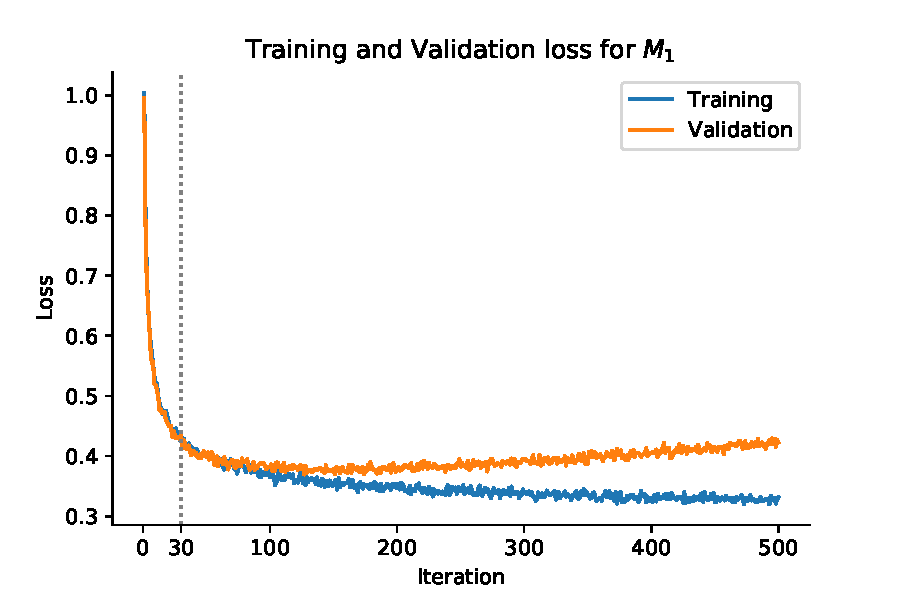
\includegraphics[width=0.95\linewidth]{figures/m1.pdf}
        \caption{Training and validation loss of a model $M_1$}
        \label{fig:m1}
    \end{subfigure}
    \centering
    \begin{subfigure}[b]{0.49\textwidth}
        \centering
        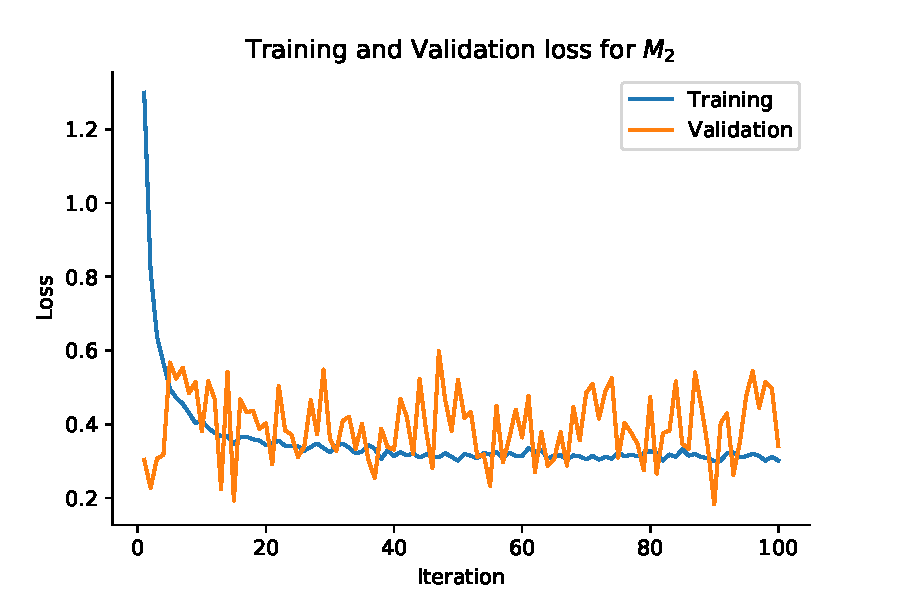
\includegraphics[width=0.95\linewidth]{figures/m2.pdf}
        \caption{Training and validation loss of a model $M_2$}
        \label{fig:m2}
    \end{subfigure}
    \caption{Example of training curves showing training and validation loss for two hypothetical models $M_1$ and $M_2$.}
\end{figure}

\begin{enumerate}[1.]
\item \textbf{(6 pts)} Review the training and validation loss curve in Figure~\ref{fig:m1} (model $M_1$).
The $y$-axis shows a loss (lower is better) for the training and validation data.
The $x$-axis shows the iterations to update the model parameters (e.g. update steps on Perceptron algorithm or steps of gradient descent for logistic regression).\\
{\bf Hint:} Note that these are training curves, not learning curves.



\begin{enumerate}
\item {(\bf 3 pts)} What are the best parameters for model $M_1$? The parameters at 500 iterations or at 100 iterations? Please justify your answer.

\begin{tcolorbox}[breakable,
enhanced,
notitle,
width=14.5cm,
height=5cm]
%
% Your solution here
%

\end{tcolorbox}


\item {(\bf 3 pts)} What is the disadvantage of choosing the model with parameters obtained after 30 iterations?


\begin{tcolorbox}[breakable,
enhanced,
notitle,
width=14.5cm,
height=5cm]
%
% Your solution here
%

\end{tcolorbox}

\end{enumerate}

% ---- %
\newpage
\item \textbf{(4 pts)} Review the training and validation loss curve in Figure~\ref{fig:m2} of model $M_2$. 

Which of the following explanations and decisions are appropriate for the observed behavior in \ref{fig:m2}?\\
{\bf Choose all answers that are correct. You don't need to justify your answer.}
\begin{enumerate}[(A)]
    \item The validation data is scarce and not very representative.
    \item The model has not converged yet at 100 iterations and many more iterations will likely improve the training loss.
    \item Getting more validation data will not reduce the training loss.
    \item The training loss has converged, so obtaining more and better training data will not reduce the training loss further.
\end{enumerate}

\begin{tcolorbox}[breakable,
enhanced,
notitle,
width=15.1cm,
height=5cm]
%
% Your solution here
%

\end{tcolorbox}

\item \textbf{(4 pts)} Which statement about $k$-fold cross validation is incorrect?\\
{\bf Choose all answers that are correct.}
\begin{enumerate}[(A)]
    \item With larger $k$, the training set gets larger, while the test set gets smaller.
    \item When splitting data into folds, it is desirable to minimize the variance across folds.
    \item When using $k$-fold cross validation, using a smaller $k$ means it will take more time to run the evaluation.
    \item When $k=N$, where $N$ is the size of the data set, $k$-fold cross validation is the same as leave-one-out cross validation.
\end{enumerate}

\begin{tcolorbox}[breakable,
enhanced,
notitle,
width=15.1cm,
height=5cm]
%
% Your solution here
%

\end{tcolorbox}

\newpage
\item \textbf{(6 pts)} Given the supervised learning dataset with 3 training examples $(X_1,Y_1) =(0,1)$, $(X_2,Y_2)=(1,1)$, $(X_3,Y_3) = (2,-1)$, use the Perceptron algorithm to learn a classifier. If needed, use $\text{sign}(0)=1$.  The Perceptron classifier will have two parameters $w=(w_0, w_1)$ (the first parameter, $w_0$ acts as the bias).
What is the average 0-1 loss of the Perceptron algorithm evaluated by 3-fold cross validation? (Please also describe, for each fold/iteration of the cross validation, what is the training data used and the loss obtained).

\emph{
Note: Without a bias term for the Perceptron, the data may not be linearly separable. 
As we saw in class, a simple way to add a bias term to a linear classifier is to add an extra feature with value of 1 for all data points.
This way, the new data points become $X'=\{(0, 1), (1, 1), (2, 1)\}$. 
}



\begin{tcolorbox}[breakable,
enhanced,
notitle,
width=15.5cm,
height=18cm]
%
% Your solution here
%

\end{tcolorbox}

\end{enumerate}


\newpage

\question{14} {\bf \large Ensemble methods (AdaBoost)}


Consider the dataset in the following table:

\begin{table}[h!]
	\centering
	\begin{tabular}{c|cc|c}
		\toprule
		\textbf{Index} $(i)$ & \textbf{Feature 1} $(X_{i1})$ & \textbf{Feature 2} $(X_{i2})$ & \textbf{Class label} $(y_i)$\\
		\midrule
		1 & -1 &  1 & +1 \\
		2 &  1 &  1 & -1 \\
		3 &  1 & -1 & +1 \\
		4 & -1 & -1 & +1 \\
		\bottomrule
	\end{tabular}
\end{table}

For this question, you have to show the first few steps of the AdaBoost algorithm.
The weak learner can be one of the four possible decision stumps illustrated in Fig. \ref{fig:stumps} (i.e., at each step you must choose one of the classifiers in the figure, to minimize the weighted empirical error rate, defined as COMPLETE HERE, breaking any ties by choosing the classifier with lower number).

\begin{figure}[h!]
	\centering
	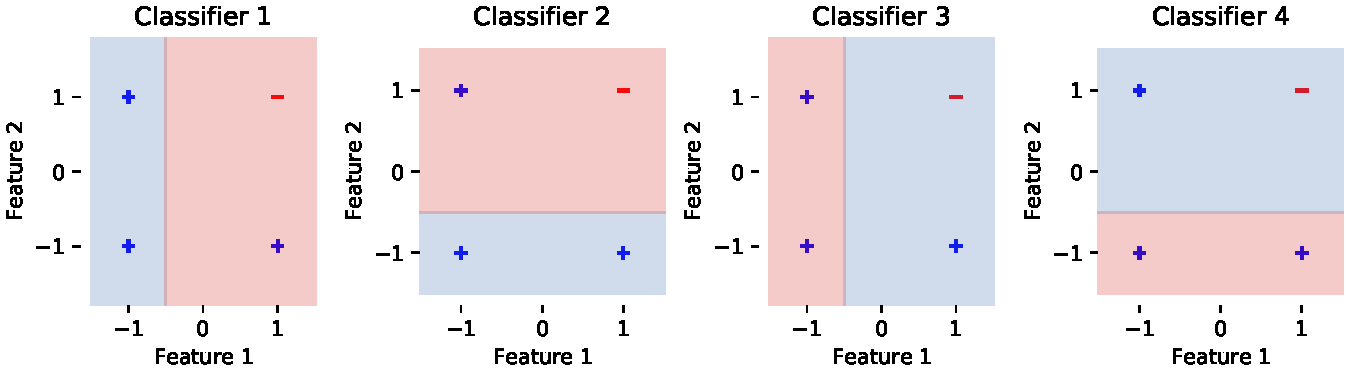
\includegraphics[width=0.9\textwidth]{figures/stumps.pdf}
	\caption{Choices of classifiers for the dataset. The solid red areas are assigned label $-1$ and the hatched blue areas are assigned label $+1$}
	\label{fig:stumps}
\end{figure}

\FloatBarrier
\begin{enumerate}
	\item \textbf{(6 pts)} Complete the following table, with the correct values computed during the execution of the AdaBoost algorithm, for $t=1, \dots, 5$. Please refer to lecture slides for details of AdaBoost.
\begin{table}[h!]
	\centering
	\begin{tabular}{c| cc | cccc | c | cccc}
		\toprule
			 & & & \multicolumn{4}{c|}{$D_t(i)$} & $h_t$ & \multicolumn{4}{c}{$\mathbb{I}(h_t(\ux_i) \neq y_i)$} \\
			$t$ & 
			$\xi_t$ & 
			$\alpha_t$ & 
			$i=1$ & $i=2$ & $i=3$ & $i=4$  &
			Classifier &
			$i=1$ & $i=2$ & $i=3$ & $i=4$ \\
		\midrule
		1 &  &  &&& & & &&& \\
		2 &  &  &&& & & &&& \\
		3 &  &  &&& & & &&& \\
		4 &  &  &&& & & &&& \\
		5 &  &  &&& & & &&& \\
		\bottomrule
		
	\end{tabular}
\end{table}


\FloatBarrier
\item \textbf{(4 pts)} Complete the following table, with the predictions computed by the AdaBoost algorithm for the training data, at the end of training (i.e. after $T=5$ rounds).
\begin{center}
	\begin{tabular}{ccccc}
		\toprule
		& \multicolumn{4}{c}{$\hat{h}(\ux_i)$} \\
		& $i=1$ & $i=2$ & $i=3$ & $i=4$ \\
		\midrule
		$\sum_{t=1}^T\alpha_t h(\ux_i)$&        &       &       &       \\
		$\hat{h}(\ux_i)$ &       &       &       &       \\
		\bottomrule
	\end{tabular}
\end{center}


\newpage
\item \textbf{(4 pts)} Assuming we stopped the algorithm after finishing the step $t=4$, what is the predicted label for a new sample $\underline{x} = (0, -1)$? If the true label of this new test example is $+1$, what is the 0-1 loss for this example?

\begin{tcolorbox}[breakable,
enhanced,
notitle,
width=16.1cm,
height=7cm]
%
% Your solution here
%

\end{tcolorbox}
\end{enumerate}


\newpage
\question{20} {\bf \large SVM}

Consider an SVM that obtains a decision boundary through the maximization optimization in Equation (\ref{eq:hard_svm}), which is equivalent to the minimization optimization in Equation (\ref{eq:hard_svm_min}), where $\beta$ and $\beta_0$  denote the parameters, $x_i$ the $i$-th training example, $y_i \in \{-1, 1\}$ the class label for the $i$-th training example, $M$ the margin, $N$ the number of instances.


\begin{equation}
\begin{aligned}
\label{eq:hard_svm}
&\max _{\beta, \beta_0,\|\beta\|_{2}=1} M \\
\text{subject to   }\text{  } y_i&\left(x_i^T \beta+\beta_0\right) \geq M,\; i=1, \ldots, N.
\end{aligned}
\end{equation}


which is equivalent to


\begin{equation}
\label{eq:hard_svm_min}
\begin{aligned}
&\min _{\beta, \beta_0} \frac{1}{2}\|\beta\|_{2}^2\\
\text{subject to   }\text{  }   & y_i\left(x_i^T \beta+\beta_0\right) \geq 1,\;i=1, \ldots, N.
\end{aligned}
\end{equation}



Mark true or false for the following assertions (Q4.1, Q4.2, Q4.3) and justify your answer. Questions with no justification will receive 0 points. 

\begin{enumerate}[1.]

\item {\bf (4 pts)} This SVM objective assumes data is linearly separable. 
        
        
\begin{tcolorbox}[breakable,
enhanced,
notitle,
width=16.6cm,
height=3cm]
%
% Your solution here
%
\end{tcolorbox}

        
\item {\bf (4 pts)} After obtaining the decision boundary in Equation \ref{eq:hard_svm}, if we modify $\beta$ while maintaining the restriction $\|\beta\|^2_{2}=1$, this would modify the minimum distance from the decision boundary to the origin. 

\begin{tcolorbox}[breakable,
enhanced,
notitle,
width=16.6cm,
height=3cm]

%
% Your solution here
%
\end{tcolorbox}

\item {\bf (4 pts)} Assume the maximum margin obtained by the model was $M=4 = d_1 + d_2$, where  $d_1=2$ and $d_2=2$ denote the distance from the decision boundary to hyperplanes $H_1$ and $H_2$ defined by the support vectors. If we add 1 to $\beta_0$, the new maximum margin would be $M+1$.

\begin{tcolorbox}[breakable,
enhanced,
notitle,
width=16.6cm,
height=3cm]  
%
% Your solution here
%
\end{tcolorbox}
        
        
\item {\bf (4 pts)} {\bf  SVM decision boundary.}
Consider again an SVM whose decision boundary is obtained by Equations \ref{eq:hard_svm} and 
 \ref{eq:hard_svm_min} like in the previous questions. Now, consider the training dataset with two training classes (signaled as squares and triangles) given by the scatter plot in the following figure. Draw the decision boundary for this dataset obtained by our SVM on it. The drawing needs to correctly separate the examples but there are multiple possible solutions. Each point of the line you draw must match the points of the true decision boundary within the error margin of 10 unit intervals along the $x$-axis and $y$-axis. 
 \begin{tcolorbox}[breakable,
enhanced,
notitle,
width=15.8cm,
height=15cm]  
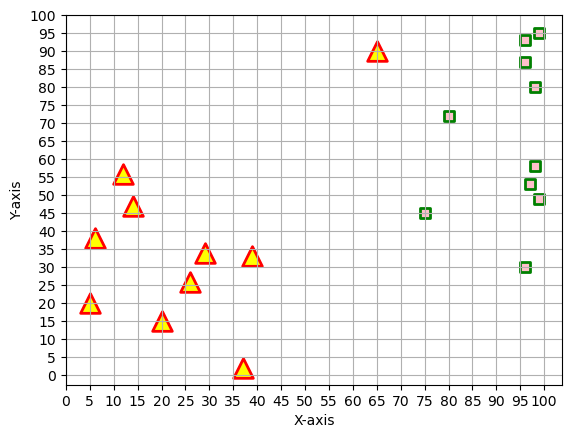
\includegraphics[width=1
\linewidth]{./figures/svm_graph1.png}
\end{tcolorbox}

\newpage

\item {\bf (4 pts)} {\bf  SVM decision boundary with removed example.} Now pick a single data point $\mathbf{x}_i$ that, if removed, would yield the maximum possible increase in the margin of a new SVM decision boundary over the dataset without $\mathbf{x}_i$. Indicate which point is $\mathbf{x}_i$ in the figure below (reproduction of last question). Draw the new decision boundary after $\mathbf{x}_i$'s removal on it. The drawing needs to correctly separate the remaining examples but there are multiple possible solutions. Each point of the line you draw must match the points of the true new decision boundary within the error margin of 10 unit intervals along the $x$-axis and $y$-axis.
 
 \begin{tcolorbox}[breakable,
enhanced,
notitle,
width=15.8cm,
height=15cm]  
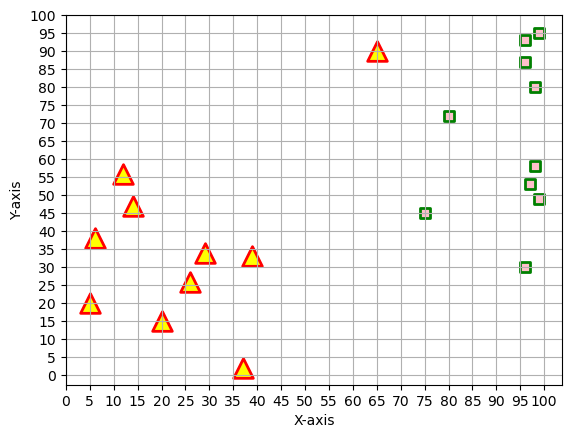
\includegraphics[width=1
\linewidth]{./figures/svm_graph1.png}
\end{tcolorbox}
 
 

\end{enumerate}












\newpage

\section*{Programming Part (20+18=38 pts)}

There are some basic requirements that you should follow when you submit your code:
\begin{itemize}
\item Make sure you don't import any package that you are allowed.
\item Make sure your returned data type follows the given data type.
\item Make sure your code does not contain \texttt{matplotlib} popups, such as \texttt{plt.show()}.
\end{itemize}

\question{20}{\bf \large Cross-Validation}

In this assignment, you will use a $k$-fold cross validation technique to measure the performances and tune hyperparameters of some algorithms that you have learned or implemented, including KNN, Decision Tree, Logistic Regression and SVM. You will still be using the dating dataset that you have seen in HW2. Again, it is a part of the whole dataset, while the test data is not published to you and will be used for grading. Please refer to the previous homework if you have questions about datasets.

A $k$-fold cross-validation is implemented as follows.

\begin{center}
    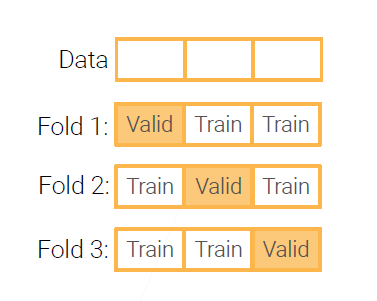
\includegraphics[width=4cm]{./figures/cv.png}
\end{center}


\begin{itemize}
    \item Partition the training data into $k$ parts.
    \item For $i=1, \dots, k$: use the $i$-th part as the validation set and the rest for training
    \item Report the validation error averaged over $k$ rounds.
    
\end{itemize}

\rightline{\href{https://c.d2l.ai/stanford-cs329p/_static/pdfs/cs329p_slides_6_3.pdf}{(Huang, Li and Smola, 2021)}}

\subsubsection*{1. Implementation}

Implement the required functions in the file \verb|cross_validation.py|:
\begin{enumerate}[(a)]
    \item \textbf{(3 pts)} Implement \verb|create_folds()| method, which takes in data samples \verb|X| and their labels \verb|y|. You should partition the data into $k$-folds and return a list of tuples of \verb|(X, y)| with each element in the tuple being a fold. Please refer to the code comments for a sample output.
    \item \textbf{(3 pts)} Implement \verb|train_valid_split()| method, which takes in a list of folds and an integer index at which the fold will be used as the validation set. Combine the rest of the folds to get the training set. Return two tuples: (\verb|X_train|, \verb|y_train|), (\verb|X_val|, and \verb|y_val|). Please refer to the code comments for a sample output.
    \item \textbf{(3 pts)} Implement \verb|cross_val_score()| method, which takes in data samples \verb|X|, their labels \verb|y|, and a classifier \verb|clf| as input, and should return two lists: \verb|train_accs| and \verb|val_accs|, where each element represents the accuracy of the training or validation dataset of a specific folds split case. Please refer to the code comments for a sample output.
\end{enumerate}
Implement the required functions in the file \verb|evaluation.py|:
\begin{enumerate}[(a)]\addtocounter{enumi}{3}
    \item {(\bf 3 pts)} Implement \verb|find_best_param| method, which uses $k$-fold cross validation to find the best parameter of a model. Models can be Logistic Regression, Decision Tree and SVM. It takes the pre-processed dataset \verb|(X, y)|, the number of folds \verb|k|, the model name (\verb|`logistic', `decision_tree'| or \verb|`svm'|), and the corresponding parameters as input, and should return the training and validation accuracy dictionaries and also the best parameter.
    \begin{itemize}
        \item For Logistic Regression model, you will be using the previous code and tune the hyperparameter \verb|lr| (learning rate).
        \item For Decision Tree, you will be using the sklearn library, \verb|sklearn.tree.DecisionTreeClassifier|, and tune the hyperparameter \verb|max_depth|.
        \item For SVM, you will be using the sklearn library \verb|sklearn.svm.LinearSVC|, which is a linear SVM, and tune the hyperparameter $C$, which is a regularization parameter, and basically determines the influence of misclassification on the data samples. The larger the value of $C$ is, the less tolerant your model will be to misclassified samples.
    \end{itemize}
Please refer to the code comments for a sample output.
\end{enumerate}

\paragraph{2. Evaluation}~\\

This part is simple. We have implemented many functions for you, including the plotting of learning curves, cross validation processes and the main function. Please refer to the code for more details. If your implementations are correct, you will be able to get all the results. What you need to do is just attaching your results to the final report.
\begin{enumerate}[(a)]
\item {\bf (2 pts)} Print out your best parameters for the three models that you tuned by using k-fold cross validation. The format of your output should be:\\ \\
    \texttt{
    The best learning rate for Logistic Regression is ...}\\
    \texttt{
    The best max\_depth for Decision Tree is ...}\\
    \texttt{
    The best C for SVM is ...}
 \begin{tcolorbox}[breakable,
enhanced,
notitle,
width=15.8cm,
height=5cm]  

\end{tcolorbox}

\item {\bf (6 pts)} Attach the learning curves of Logistic Regression, DecisionTree, and SVM in your report, which can be automatically generated under your working directory (3 figures). Briefly dicuss your observations.

 \begin{tcolorbox}[breakable,
enhanced,
notitle,
width=15.8cm,
height=24cm]  
\end{tcolorbox}

\end{enumerate}
\newpage
\question{18}{\bf \large Bagging and Boosting}

Bagging is generally used to help stabilize classifiers with unstable learning algorithms (optimal score searching algorithms). A classifier has a stable learning algorithm if, by changing the training data, the predicted class labels in the test data don't change. 
For instance, the predictions of a decision tree might significantly change with a small change in the training data. 
This definition depends on the amount of data, of course. Classifiers that are unstable with $10^3$ training examples may be stable with $10^{9}$ examples.
Bagging works by aggregating the answers of unstable classifiers trained over multiple training datasets. These multiple datasets are often not independent, generally sampled with replacement from the same training data. 

Boosting works by converting weak classifier (very simple models) to strong ones (models that can describe complex relationships between the inputs and the class labels).
A weak learner is a classifier whose output of an test example attributes $x_i$ is only slightly correlated with its true class $t_i$. That is, the weak learner classifies the data better than random, but not much better than random.
In boosting, weak learners are trained sequentially in a way that the current learner gives more emphasis to the examples that past learns made mistakes on.

\begin{enumerate}[1.]
\item {\bf (8 pts)} Suppose we decide to use a large deep feedforward network as a classifier with a small training dataset. Assume the network can perfectly fit the training data but we want to make sure it is accurate in our test data (without having access to the test data). Would you use boosting or bagging to help improve the classification accuracy? Describe what would be the problem of using the other approach.
  \begin{tcolorbox}[breakable,
        enhanced,
        notitle,
        width=15.3cm,
        height=8cm]
%
% Your solution here
%
        \end{tcolorbox}
        \newpage
\item {\bf (10 pts)} Download the code at \href{https://www.dropbox.com/s/swdrapsebhad6tb/mistery_classifier.zip?dl=0}{mistery\_classifier.zip} . Read the code and answer the following questions:\\
{\bf Note:}  You don't need to run the code, but if you want to run it on the scholar.rcac.purdue.edu cluster, you will need to command \texttt{module load anaconda/5.1.0-py36} \\
   \begin{enumerate}[(a)]
   \item {\bf (5 pts)} Which classifier is this? Why are the trees used in this classifier so shallow? Describe how the classifier works using pseudo-code. \\
   {\bf Hint:} It uses decision trees but this is not a decision tree classifier.
      \begin{tcolorbox}[breakable,
        enhanced,
        notitle,
        width=15cm,
        height=8cm]
%
% Your solution here
%
        \end{tcolorbox}
        %\newpage
   \item {\bf (5 pts)} What happens if we have mislabeled data? Why mislabeled data could be a problem?\\
   {\bf Hint:} We are looking for an answer that uses the training weights of the examples at each iteration as a justification.
         \begin{tcolorbox}[breakable,
        enhanced,
        notitle,
        width=15cm,
        height=6cm]
%
% Your solution here
%
        \end{tcolorbox}
  \end{enumerate}
 
\end{enumerate}


\newpage

\subsection*{Submission Instructions}

Please read the instructions carefully. Failing to follow any part might incur some score deductions.


\subsubsection*{1. PDF upload}
Your report should be {\bf one} a PDF file or multiple image files. Please only upload multiple image files if you are very familiar with Gradescope.

{\bf Important: Associate the Gradescope questions with your upload no matter it is a PDF or multiple images. TAs have the right to give zero points if it is not clear where the answer to a question is because it was not linked on Gradescope.}

As stated at the beginning, please remember that {\bf clarity and conciseness} will be rewarded.

There are some suggestions (but not limited to) that you can write the PDF report:
\begin{enumerate}[1)]
\item Print out the PDF, use your pens to write in real paper, scan or take photos, combine these photos into a MS Word file, and print as PDF. It is recommended to scan using some apps, like \textit{Notes} on iOS and \textit{Adobe Scan} on Android, because this will make images clearer than solely taking photos. (Of course if you want to use a scanner).
    \item Use electronic devices (like iPad) and pens (like Apple pencil), write your solutions in the given grey colored text boxes, and export to PDF. If you are very familiar with Gradescope, you can try to upload pictures directly.
    \item Write your answers in the given \verb|.tex| file and export to PDF.
\end{enumerate}

If you decide to upload multiple images, {\bf please scan them before uploading} (check suggestion 1) above), because photos are not easy to grade. {\bf TAs have the right to give zero points if your submission is not readable.}

The report PDF must be {\bf uploaded on Gradescope} (see link at Brightspace)


\subsubsection*{2. Code Upload}



\noindent \textbf{Naming convention}: \texttt{[your\_username]\_hw\homeworknumber}

All your submitting code files should be included in one folder. The folder should be named with the above naming convention. For example, if my username is ``\texttt{smith}'', then for Homework \homeworknumber, my folder name should be ``\texttt{smith\_hw\homeworknumber}''. 


The \textbf{folder structure} should be {\bf exactly the same} as the following directory tree:

\dirtree{%
.1 smith\_hw\homeworknumber.
.2 cross\_validation.py.
.2 dating\_train.csv.
.2 evaluation.py.
.2 logistic\_regression.py.
.2 utils.py.
}
It is ok if you include your plotted figures in your folder. 
 
\textbf{{\color{red} We noticed that there are some unqualified submissions of previous homework assignments:
\begin{itemize}
    \item Some of you put all your code files into the original \texttt{hw\#\_code} folder that you were given. Some even included the \texttt{hw\#\_handout} folder which contains the PDF and latex handouts.
    \item Some of you used PyCharm to develop your code and included the \texttt{venv} folder in your submission. This made your submission extremely large.
\end{itemize}
These cases made it hard for our autograding script hard to find your code and had to give your code 0 point. Let us restate, all of your code files should be directly put into a folder called \texttt{[your\_username]\_hw\#}, which should not contain any subfolder. After this, you can do (1) either transfer the \texttt{[your\_username]\_hw\#} folder to data.cs and compress your folder on it, or (2) compress your folder first then transfer it to data.cs and use \texttt{turnin} command to submit. From HW3, We will give 0 credit to those submissions that are against the requirements and will not accept regrading request.}
}

\hfill


\noindent \textbf{Use the following command to compress your folder}:

\textbf{\texttt{tar -czvf [your\_username]\_hw\homeworknumber.tar.gz  [your\_username]\_hw\homeworknumber}} 


\hfill

%\newpage
\noindent \textbf{Submit the code}: 
{\bf TURNIN Instructions}

Please submit your compressed file on \texttt{data.cs.purdue.edu} by turnin command line, e.g. 

\texttt{turnin -c cs373 -p HW\homeworknumber{} [your\_username]\_hw\homeworknumber.tar.gz}

Please check the following notes before you submit your code:
\begin{itemize}
    \item Please make sure you didn't use any library/source explicitly forbidden to use. If such library/source code is used, you will get 0 pt for the coding part of the assignment. 
    \item {\bf If your code doesn't run on \texttt{scholar.rcac.purdue.edu}, then even if it compiles in another computer, your code will still be considered not-running and the respective part of the assignment will receive 0 pt.}
\end{itemize}

\end{document}

